\chapter{ỨNG DỤNG CÂY QUYẾT ĐỊNH (DECISION TREE)
CHO BÀI TOÁN PHÂN LOẠI VỚI SCIKIT-LEARN}

\section{Tập dữ liệu hoa Iris (Iris flower dataset)}
Iris flower dataset là một bộ dữ liệu nhỏ. Bộ dữ liệu này bao gồm
thông tin của ba loại hoa Iris (một loài hoa lan) khác nhau:
Iris setosa, Iris virginica và Iris versicolor.

Mỗi loại có 50 bông hoa được đo với dữ liệu là 4 thông tin:
chiều dài, chiều rộng đài hoa (sepal), và chiều dài, chiều rộng cánh hoa (petal).

Hình \ref{fig:iris} là ví dụ về hình ảnh của ba loại hoa.

\begin{figure}[h!]
    \centering
    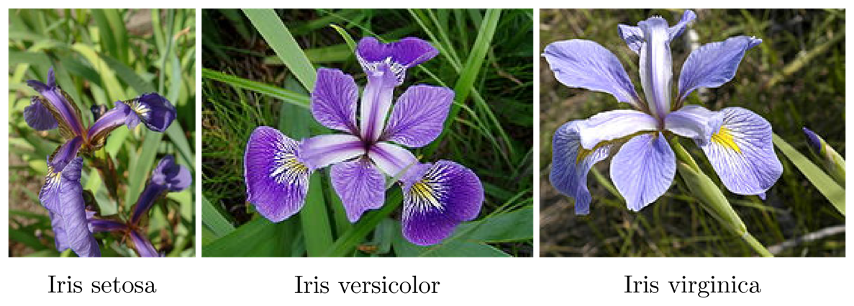
\includegraphics[width=0.7\textwidth]{thesis/decision-tree/app/iris.png}
    \caption{Ví dụ về Iris flower dataset}
    \label{fig:iris}
\end{figure}

Bộ dữ liệu nhỏ này thường được sử dụng trong nhiều thuật toán
Machine Learning trong các lớp học.

\section{Xây dựng mô hình}

\subsection{Import thư viện và tập dữ liệu:}

Trước tiên, chúng ta cần khai báo vài thư viện và load dữ liệu Iris flower dataset.

Vì tệp ở định dạng CSV, nên sử dụng phương thức read\_csv của panda để đọc tệp dữ liệu CSV.

\begin{lstlisting}[language=Python]
import pandas as pd
import numpy as np
# load data
dataset = pd.read_csv('Iris.csv')
\end{lstlisting}

\subsection{Phân tích dữ liệu:}

Thực thi lệnh sau để xem số hàng và cột trong tập dữ liệu.

\begin{lstlisting}[language=Python]
# get how many instances (rows) and how many attributes (columns)
dataset.shape
\end{lstlisting}

Kết quả đầu ra sẽ hiển thị \enquote{(150, 6)}, có nghĩa là tập dữ liệu
có 150 bản ghi và 6 thuộc tính.

Thực thi lệnh sau để xem các thông tin cơ bản:
giá trị cột dữ liệu lớn nhất, nhỏ nhất, và trung bình.

\begin{lstlisting}[language=Python]
# show basic info: max, min, mean of dataset columns
dataset.describe()
\end{lstlisting}

Kết quả đầu ra như bảng dưới.

\begin{terminaloutput}
      Id         SepalLengthCm SepalWidthCm PetalLengthCm PetalWidthCm
count 150.000000 150.000000    150.000000   150.000000    150.000000
mean  75.500000  5.843333      3.054000     3.758667      1.198667
std   43.445368  0.828066      0.433594     1.764420      0.763161
min   1.000000   4.300000      2.000000     1.000000      0.100000
25%   38.250000  5.100000      2.800000     1.600000      0.300000
50%   75.500000  5.800000      3.000000     4.350000      1.300000
75%   112.750000 6.400000      3.300000     5.100000      1.800000
max   150.000000 7.900000      4.400000     6.900000      2.500000
\end{terminaloutput}

Thực thi lệnh sau để xem dữ liệu thống kê của các cột (bao gồm các cột phân loại).

\begin{lstlisting}[language=Python]
# display statistical data of columns (including categorical columns)
dataset.describe(include = 'all')
\end{lstlisting}

Kết quả đầu ra như bảng dưới.

\begin{terminaloutput}
       Id         SepalLengthCm SepalWidthCm PetalLengthCm PetalWidthCm Species
count  150.000000 150.000000    150.000000   150.000000    150.000000   150
unique NaN        NaN           NaN          NaN           NaN          3
top    NaN        NaN           NaN          NaN           NaN          Iris-setosa
freq   NaN        NaN           NaN          NaN           NaN          50
mean   75.500000  5.843333      3.054000     3.758667      1.198667     NaN
std    43.445368  0.828066      0.433594     1.764420      0.763161     NaN
min    1.000000   4.300000      2.000000     1.000000      0.100000     NaN
25%    38.250000  5.100000      2.800000     1.600000      0.300000     NaN
50%    75.500000  5.800000      3.000000     4.350000      1.300000     NaN
75%    112.750000 6.400000      3.300000     5.100000      1.800000     NaN
max    150.000000 7.900000      4.400000     6.900000      2.500000     NaN
\end{terminaloutput}

Thực thi lệnh sau để kiểm tra năm bản ghi đầu tiên của tập dữ liệu.

\begin{lstlisting}[language=Python]
# show some first rows
dataset.head(5)
\end{lstlisting}

Kết quả đầu ra như bảng dưới.

\begin{terminaloutput}
  Id SepalLengthCm SepalWidthCm PetalLengthCm PetalWidthCm Species
0 1  5.1           3.5          1.4           0.2          Iris-setosa
1 2  4.9           3.0          1.4           0.2          Iris-setosa
2 3  4.7           3.2          1.3           0.2          Iris-setosa
3 4  4.6           3.1          1.5           0.2          Iris-setosa
4 5  5.0           3.6          1.4           0.2          Iris-setosa
\end{terminaloutput}

Thực thi lệnh sau để kiểm tra năm bản ghi cuối của tập dữ liệu.

\begin{lstlisting}[language=Python]
# show some last rows
dataset.tail(5)
\end{lstlisting}

Kết quả đầu ra như bảng dưới.

\begin{terminaloutput}
    Id  SepalLengthCm SepalWidthCm PetalLengthCm PetalWidthCm Species
145 146 6.7           3.0          5.2           2.3          Iris-virginica
146 147 6.3           2.5          5.0           1.9          Iris-virginica
147 148 6.5           3.0          5.2           2.0          Iris-virginica
148 149 6.2           3.4          5.4           2.3          Iris-virginica
149 150 5.9           3.0          5.1           1.8          Iris-virginica
\end{terminaloutput}

Thực thi lệnh sau để xem số lượng instance (hàng) thuộc về từng lớp.

\begin{lstlisting}[language=Python]
# numbers of instances (rows) that belong to each class.
dataset.groupby('Species').size()
\end{lstlisting}

Kết quả đầu ra như bảng dưới. Thấy được, mỗi loại hoa đều có 50 mẫu.

\begin{terminaloutput}
Species
Iris-setosa        50
Iris-versicolor    50
Iris-virginica     50
dtype: int64
\end{terminaloutput}

\subsection{Tiền xử lý dữ liệu:}

Trong phần này, chúng ta chia dữ liệu của mình thành các thuộc tính và nhãn,
sau đó sẽ chia dữ liệu kết quả thành cả tập huấn luyện và tập kiểm tra.

Bằng cách này, ta có thể huấn luyện thuật toán của mình trên
một tập dữ liệu và sau đó kiểm tra nó trên một tập dữ liệu hoàn toàn khác
mà thuật toán chưa thấy.

Điều này cung cấp cho chúng ta cái nhìn chính xác hơn về cách thuật toán
được đào tạo sẽ thực sự hoạt động như thế nào.

Để chia dữ liệu thành các thuộc tính và nhãn, thực thi đoạn mã sau.

\begin{lstlisting}[language=Python]
feature_columns = ['SepalLengthCm', 'SepalWidthCm', 'PetalLengthCm','PetalWidthCm']
X = dataset[feature_columns].values
y = dataset['Species'].values
\end{lstlisting}

Ở đây biến $X$ chứa tất cả các cột từ tập dữ liệu, ngoại trừ cột \enquote{Species},
là nhãn. Biến $y$ chứa các giá trị từ cột \enquote{Species}. Biến $X$ là tập thuộc tính
của chúng ta và biến $y$ chứa các nhãn tương ứng.

Bước tiền xử lý cuối cùng là chia dữ liệu thành các tập huấn luyện và thử nghiệm.
Thư viện model\_selection của scikit-learn chứa phương thức train\_test\_split,
chúng tôi sẽ sử dụng phương thức này để chia ngẫu nhiên dữ liệu thành
các tập huấn luyện và thử nghiệm.

\begin{lstlisting}[language=Python]
from sklearn.model_selection import train_test_split
X_train, X_test, y_train, y_test = train_test_split(X, y, test_size = 0.3, random_state = 0)
\end{lstlisting}

Trong đoạn mã trên, tham số test\_size chỉ định tỷ lệ của tập thử nghiệm,
ở đây sử dụng 30\% dữ liệu cho tập thử nghiệm và 70\% cho tập huấn luyện.

\subsection{Đào tạo và đưa ra dự đoán:}

Khi dữ liệu đã được chia thành các tập huấn luyện và thử nghiệm,
bước cuối cùng là huấn luyện thuật toán Decision Tree trên dữ liệu này và
đưa ra dự đoán. Scikit-learn chứa các class/phương thức tích hợp sẵn
cho các thuật toán Decision Tree khác nhau.

Để sử dụng cho bài toán phân loại, sử dụng class $DecisionTreeClassifier$.
Phương thức $fit$ của class này được gọi để huấn luyện thuật toán
trên dữ liệu huấn luyện, được truyền dưới dạng tham số cho phương thức $fit$.

Ngoài ra, ở đây ta sử dụng hai độ đo khác nhau, là \enquote{Gini} và
\enquote{Entropy}, tạo ra hai mô hình khác nhau.

\subsubsection{criterion=\enquote{gini}}
Thực thi tập lệnh sau để huấn luyện thuật toán.

\begin{lstlisting}[language=Python]
from sklearn.tree import DecisionTreeClassifier
dt = DecisionTreeClassifier(criterion='gini')
dt.fit(X_train, y_train)
\end{lstlisting}

Bây giờ bộ phân loại đã được đào tạo, hãy đưa ra dự đoán
trên dữ liệu thử nghiệm.
Để đưa ra dự đoán, phương pháp dự đoán của lớp $DecisionTreeClassifier$
được sử dụng. Hãy xem đoạn mã sau để sử dụng.

\begin{lstlisting}[language=Python]
y_pred_dt = dt.predict(X_test)
\end{lstlisting}

\textbf{Đánh giá thuật toán:}
Tại thời điểm này, chúng ta đã đào tạo thuật toán của mình và đưa ra
một số dự đoán. Bây giờ chúng ta sẽ xem thuật toán chính xác đến mức nào.

Đối với các nhiệm vụ phân loại, một số chỉ số thường được sử dụng
là ma trận nhầm lẫn, độ chính xác, thu hồi và điểm F1.

Thư viện của scikit-learn chứa phương thức classification\_report và
confusion\_matrix có thể được sử dụng để tính toán các số liệu này.

\begin{lstlisting}[language=Python]
from sklearn.metrics import classification_report, confusion_matrix
print(confusion_matrix(y_test, y_pred_dt))
print(classification_report(y_test, y_pred_dt))
dt_score = dt.score(X_test, y_test)
print(f"Decision Tree classifier accuracy score is %.2f" % dt_score)
\end{lstlisting}

Kết quả như bên dưới.

\begin{terminaloutput}
[[16  0  0]
[ 0 17  1]
[ 0  0 11]]
                 precision    recall  f1-score   support

    Iris-setosa       1.00      1.00      1.00        16
Iris-versicolor       1.00      0.94      0.97        18
 Iris-virginica       0.92      1.00      0.96        11

       accuracy                           0.98        45
      macro avg       0.97      0.98      0.98        45
   weighted avg       0.98      0.98      0.98        45

Decision Tree classifier accuracy score is 0.98
\end{terminaloutput}

Từ confusion\_matrix, có thể thấy rằng trong số 45 trường hợp
thử nghiệm, thuật toán chỉ phân loại sai 1. Đây là độ chính xác 98\%.

\subsubsection{criterion=\enquote{entropy}}
Thực thi tập lệnh sau để huấn luyện thuật toán.

\begin{lstlisting}[language=Python]
from sklearn.tree import DecisionTreeClassifier
dt = DecisionTreeClassifier(criterion='entropy')
dt.fit(X_train, y_train)
\end{lstlisting}

Dự đoán trên dữ liệu thử nghiệm.

\begin{lstlisting}[language=Python]
y_pred_dt = dt.predict(X_test)
\end{lstlisting}

\textbf{Đánh giá thuật toán:}

\begin{lstlisting}[language=Python]
from sklearn.metrics import classification_report, confusion_matrix
print(confusion_matrix(y_test, y_pred_dt))
print(classification_report(y_test, y_pred_dt))
dt_score = dt.score(X_test, y_test)
print(f"Decision Tree classifier accuracy score is %.2f" % dt_score)
\end{lstlisting}

Kết quả như bên dưới.

\begin{terminaloutput}
[[16  0  0]
[ 0 17  1]
[ 0  0 11]]
                 precision    recall  f1-score   support

    Iris-setosa       1.00      1.00      1.00        16
Iris-versicolor       1.00      0.94      0.97        18
 Iris-virginica       0.92      1.00      0.96        11

       accuracy                           0.98        45
      macro avg       0.97      0.98      0.98        45
   weighted avg       0.98      0.98      0.98        45

Decision Tree classifier accuracy score is 0.98
\end{terminaloutput}

Kết quả không khác gì so với sử dụng độ đo \enquote{Gini}.
